\documentclass[12pt]{report}
\usepackage{graphicx}

\title{Classification of Ailments Given Description of Symptoms}
\author{Urmzd Mukhammadnaim \\ Ben MacDonald}
\graphicspath{{./images/}}
%\bibliographystyle{apacite}

\begin{document}
\maketitle
\tableofcontents
\begin{abstract}
	In this paper, we address the challenges experienced in the preliminary research phase
	of ailment diagnosis performed by many individuals prior to visiting a
	healthcare professional. Due to the large quantity of varying results appearing
	once someone searches their current symptoms, we developed a Convolutional
	Neural Network (CNN) that reduces this clutter by returning only the most
	probable medical condition given the user’s description. Forthcoming, we
	decided to limit the possible classifications to the medical conditions,
	migraine, tetanus and depression. To train the model, data is obtained by
	scraping text data from various medical websites which were written using
	casual terminology to form a corpus. The corpus was then vectorized using
	one-hot encoding in one implementation and the FastText model in another. Once
	the model is trained, we then analyzed its ability to classify our own
	descriptions of migraines, depression and tetanus.
\end{abstract}
\chapter{Introduction}
Through the ease of access to information provided by the internet for 3.2
billion people, individuals are able to obtain data in a wide array of topics
nearly instantaneously. Among these searches are descriptions of symptoms the
user is experiencing and attempting to find a root cause for. According to a
study conducted by Eligibility, approximately 89\% of American patients search
what they are experiencing on a search engine prior to visiting their doctor.

Upon entering their symptoms, however, they will find a wide array of links to
sources such as WebMD and Mayoclinic. These pages will typically contain a
topic ailment, a description of it, a list of potential symptoms and a series
of treatments. In this current series of interactions, the user experience may
be negatively impacted by an overwhelming quantity of information. Depending on
the description, the user may observe contradicting as well as rarer and more
unlikely diagnoses. This is further exaggerated when the user enters a more
general description such as “pounding headache”, which can be attributed to a
large number of illnesses.

This problem led us to consider how to structure a process that streamlines
this preliminary research of possible diagnoses prior to visiting a medical
doctor. As opposed to using a search engine which would produce a wide range of
articles, we viewed the ideal scenario as condensing the actions to entering
the text into a model that would provide the singular most probable diagnosis.
To implement this functionality, we determined three necessary objectives:
\begin{enumerate}
	\item Acquire training and testing data that includes the description of an ailment
	\item Develop a model that produces a series of probabilities for each available ailments given data
	\item Implement this model in classifying text descriptions of a series of symptoms provided by the user
\end{enumerate}

In order to gather classified training and testing data, we scraped text from
websites which included descriptions of the ailments and its symptoms with
casual language. This was done in order to improve the likeness between the
training data and the user text the model would classify. There were several
possible approaches we could have taken to develop a model for this
multi-classification problem which we considered. Among these, we found that
Convolutional Neural Networks (CNNs) provided a flexible model which performed
well with classifying text, and has previously been used to classify symptoms
at a sentence level to a great degree of success. We were then able to observe
the network's capacity to classify training and testing data, and proceeded to
test its ability to categorize our own descriptions of any of the three
ailments.

\chapter{Related Works}
There are various ways in which we could have the user interact with the
model. Kurup and Shetty document their creation of an conversational chatbot
that utilizes Neural Networks and Decision Tree Classifiers to classify the
ailment that a particular user is experiencing given their responses to
questions about their symptoms. Due to a sparsity of publicly available
datasets, they created a JSON file with custom patterns classified by their
expected responses, and used this to train a Neural Network composed of two
dense layers, as well as dropout layers to prevent overfitting. The Decision
Tree Classifier was then trained with a dataset of binary values marking
whether or not a symptom is associated with a particular ailment. When
interacting with the Neural Network via messaging, the user could indicate
that they wished to take a “prognosis quiz”, where they would answer yes or
no to experiencing a symptom. The maximum performance of the Neural Network
reached 95\% accuracy, and the Decision Tree Classifier functioned well. This
implementation, however, does not provide a seamless series of interactions
for the user as they converse with a chatbot and, in order to classify their
symptoms, switch to a yes or no questionnaire.

Utilizing CNNs in Natural Language Processing (NLP) is growing in popularity,
with several papers documenting their efficacy in text classification. Hughes
et al describe their use of a Word2vec model and CNN to classify medical text
at the sentence level, and compare their accuracy to other NLP techniques.
Their vectorization model was trained through the use of a dataset containing
15,000 clinical research. A series of clinical articles were then each
pre-categorized as one of 26 medical categories with 4000 sentences being
randomly selected for each classification. These sentences were then vectorized
by the Word2vec model and used to train the CNN. This setup then went on to
perform with 68\% accuracy, out performing other text classification techniques
such as a bag-of-words and logistic regression model which possessed an
accuracy of 51\%. This is an effective model that displays the success of CNNs
in this context and on a larger scale with 26 individual ailments. The use of
word embeddings provides the neural network greater possible depths of
understanding for the relationships between separate words and their
associations. These benefits, however, are dependent on the large quantity of
available data to train the Word2vec model.

There is an evident distinction between classifying professional medical text
and casual descriptions with informal terminology. Gambhir et al studied the
accuracy of a Convolutional Neural Network-Long Short Term Memory (CNN-LSTM)
model in regards to monitoring social media for posts mentioning a drug name,
and classifying them as presenting personal medication intake, possible
medication intake and non-intake. In this setup, the CNN would take
vectorized training data from Word2vec and apply a series of convolution
layers and max pooling layers. The output being a series of feature maps,
this would then be input into the LSTM model, which in turn feeds data to a
series of fully connected layers and classifies the data as one of the three
possible categories. The CNN-LSTM performed with the greatest precision in
comparison to other tested models, but a lower recall than the LSTM model.
The distinction between professional medical text and casual descriptions is
an important one to make. There is a large difference between the two both in
terms of sentence structure and diction. Professional text can contain a
variety of rare terms for specific conditions which can impact a models
capacity to properly classify a description should a large corpus be
unavailable.


\chapter{Methodology}
\section{Data Collection}
One of the challenges in the endeavour was finding accessible and well
documented open-source records. As medical data is difficult to come across due
to HIPAA, PIPEDA, and other laws that bar hospitals, and other medical
organizations from distributing patient’s health documents, we had to settle
for medical encyclopedias and clinics that published articles intended for
educating individuals. To ensure baseline consistency in the data used across
the desired classifications, the descriptions were pulled from the same sites.
However, between articles on the same website, the detail in which the article
was written varied greatly. Some articles had more advertisements, others had
more miscellaneous content embedded, and most of them differed in document
structure. In other words, the data could not be accessed directly via its url
and DOM selector. The data was collected using the top-most DOM element
encapsulating all the desired information, resulting in documents with
irrelevant content within them.  As a result, a greater burden was moved onto
the preprocessor to ensure clean and usable data was entering the CNN. It
should also be noted that we used the automation library “pyppeteer” in lieu of
a simple “GET” retrieval of the html document to prevent issues accessing the
data due to Server Side Rendering (SSR). Consequently, this resulted in greater
overhead during this phase.

\section{Data Processing}
After the extraction and consequent concatenation of the documents for each
classification, we explored two preprocessor implementations. We first describe
the use of One Hot Encoder and Witten-Bell Probability Distribution to retain
morphological-level information, and generate unique sets of words that can
later be fed into the CNN. Subsequently, we analyze the use of the FastText
model as a means of retaining semantic-level information, and ensuring words
with similar words appear closer together in the subspace.

\subsection{One Hot Encoding and Witten Bell Generation}
After the documents were tokenized, the text was piped into the transformer $T1$ which applied a
series of reduction operations to remove punctuation and ultimately break the words
into their stems. The result of $T1$ consisted of a set of unique stems $D_n$
where $n$ represents the order of which the the document was processed in.
After $T1$ was applied to all documents, the union of all the sets was taken to
form the vocabulary $V$. $V$ was then fed into the \emph{FreqDist} class from
the \emph{nltk.probability} package to allow the subsequent usage of the
\emph{WittenBellProbDist} class. By allocating $|V|$ bins, and using the
\emph{FreqDist} of $D_n$, we ended up with an instance of the
\emph{WittenBellProbDist} capable of generating ${}_{V}C_{S}$ unique sets,
where $S$ represents the cardinality of the generated set. The described method
was used to prevent clustering of the same words, and ultimately prevent the
model from developing an aptitude for classifing an input based on the
frequency of its instances instead of the existence of an instance.


After $N$ samples were generated via the \emph{WittenBellProbDist} method
described above, we transformed the data using an instance of the
\emph{OneHotencoder} class fit on the the vocabulary $V$.
With this each word in $D$ had its own unique binary vector and out-of-vocabulary (OOV)
words were treated as the $0$ vector with size $|V|$.

\subsection{FastText Model}
In the alternative preprocessor, we used the FastText model. Unlike the former method,
no data generation was done. Instead, all documents were first tokenized by sentence using
an instance of the \emph{PunktSentenceTokenizer}. The sentences were then appended to
a singular file, which served as the corpus for the FastText model. Using an implementation of
the FastText model by \emph{gensim}, we trained an unsupervised word embeddings model
capable of translating words into a $R$ dimension vector.
After the FastText model was trained, each word in the vocublary was projected onto
the embedding space, resulting in vectors of cardinality $R$.

While each word had the same length, the sentence length varied. As a result,
a transformer $T_2$ was created to pad the sequence given. The algorithm
applied consisted of retrieving the vector that resulted of a coordinate-wise
max or min. Alternating between max and min operations, we injected the sequence
with the resulting vector from the operating described.

\section{Training \& Achitecture}
As there existed little data, only 20\% of the input was withheld for validation.
In this section, we describe the reasoning for the architecture we decided upon.
It should be noted that the architecture did not depend on the pre-processor.
Hence, there is no difference in the architecture of the classifier between the two implementations.

\subsection{Layers}
The primary components of the CNN consisted of 2D Convolution layers,
Max Pooling layers, a Flatten layer, Dense layers, Dropout layers and finally a Dense output layer.
The convolution layers were used as a means of determining the most critical dimensions
responsible in classfying an ailment while the max pooling layers were used to drop
dimensions with little information. After the final pooling layer, the output was
Flatten layer was used to reduce the resulting feature map onto a single column matrix, allowing it to be
transformed in later operations.
The resulting output was then passed to a series of alternating
Dense and Dropout layers. The Dense layers were added to ensure
that the CNN would  be able to fine tune its mechanisms, likely finding small details in the activation map provided
and over time, make better classifications. The Dropout layers were used to prevent overfitting
as a result of the small dataset provided. Finally, the last Dense layer was used to reduce
the learned values onto a probability distribution matching the cardinality of the classification size.

\begin{figure}[h!]
	\centering
	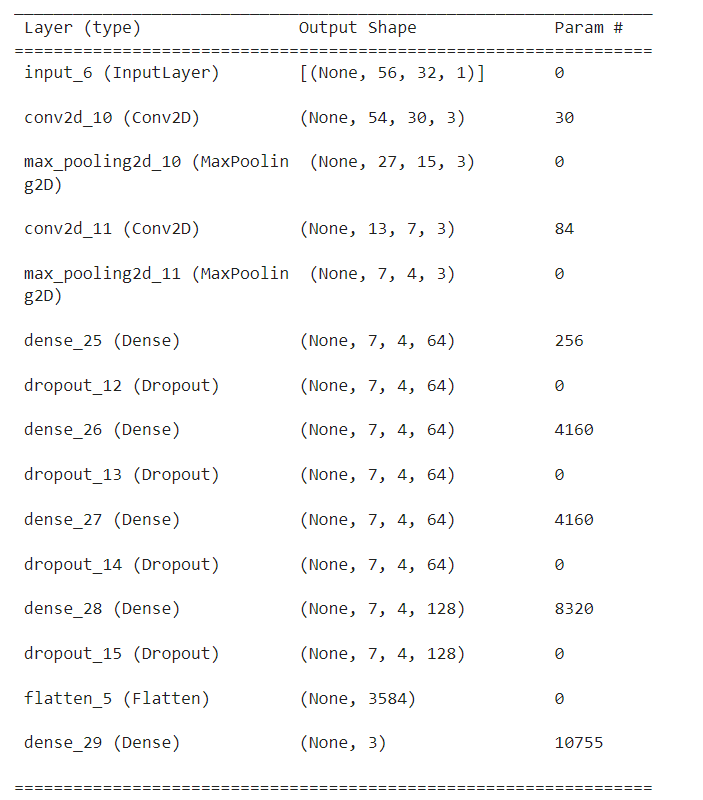
\includegraphics[ width=0.5\textwidth ]{fast-text-summary.png}
	\caption{Fast Text Model Preprocessor - CNN}
\end{figure}
\begin{figure}[h!]
	\centering
	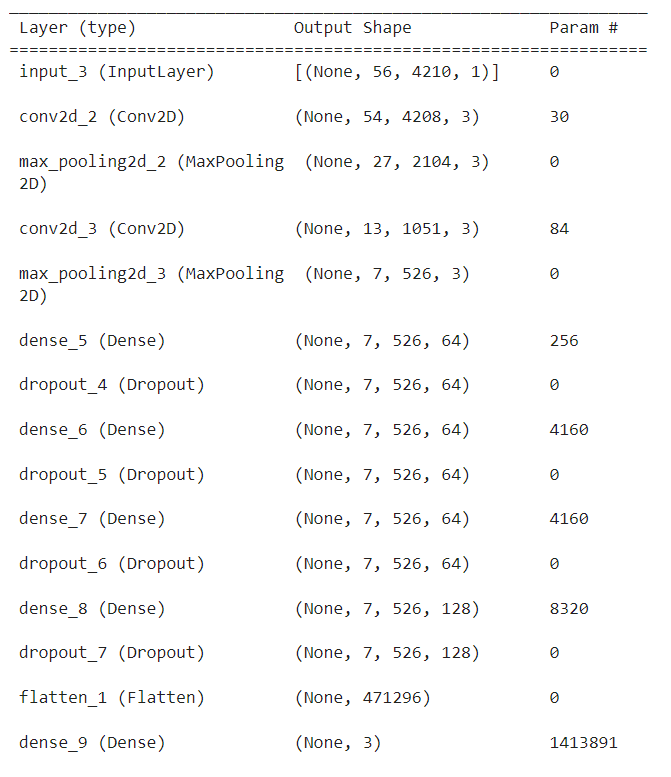
\includegraphics[ width=0.5\textwidth]{one-hot-encoder-summary.png}
	\caption{One Hot Encoding Preprocessor - CNN}
\end{figure}

\section{First Implementation}

\subsection{Discussion}
Over the course of developing the model, there were multiple changes made to the
structure and layout of the neural network and how we processed the data. In our
initial implementation, the instances for the training and test data were created
by randomly generating a series of 56 words from the scraped corpus with the use
of witten bell smoothing to include unknown words. The quantity of words was selected
based on the character length of a tweet (280) and the average character length of
English words (5). This was done due to a lack of adequate datasets which included
categorized descriptions of symptoms and their associated ailment. There are several
inherent concerns we had with this method, the most evident being the lack of contextual
meaning behind the inserted word placement and unpredictable behaviour. For the CNN, the
only pattern it would be able to recognize would be in the form of the terms fed to the
model, and it would be unable to discern semantic relationships between the words.

In order to convert the text into a matrix that the CNN would require, we first decided
upon using One Hot Encoding. This was a simple process that would convert a series of 56
words into a sparse matrix filled with zeros apart from a 1 in the word`s associated column.
Though this is an established method, it certainly impacted the performance of the model.
Since every single column represented a unique word, the dimensions of the sentence matrix
were 56x4210. This was a result of the 4210 unique stems of words in the corpus. This large
number of features slowed the model dramatically, and led to the epoch training time to increase.
We also didn`t believe this was an optimal representation of the words being used, as there was
no semantic representation through this model which would be provided through the use of word
embeddings. We would go on to use these in our second implementation of the model.

\subsection{Results}
When observing the accuracy over the number of epochs in the first implementation,
we found that at the first epoch, validation accuracy was higher than training
accuracy with values of 0.925 and 0.74 respectively. For the second epoch and onwards,
however, training accuracy varied around 0.99 and validation accuracy hovered around
0.9. \ref{fig:ohep-acc} and \ref{fig:ohep-rec}, however, are measures of how well the model performed
in regards to classifying the randomized training data. In Figure 3, we mapped the
model`s capacity to classify our written descriptions as either depression, a
migraine or tetanus.

As observed in Figure 3, the model was highly effective at classing descriptions of
depression, migraines and tetanus. Depression possessed a precision of 0.83 and a
recall of 1.0 while tetanus had a precision and recall of 1 and 0.8 respectively.
For migraines, however, the model returned a precision and recall both of 1.

There are several factors that play into the model`s ability to label these descriptions
accurately. It is evident that the neural network was capable of recognizing the particular
types of words commonly used when describing the three illnesses as scraped from medical
websites. An example of an accurately labelled symptom description tested was "my head
feels like it's spinning, pain in head, pounding throbbing". Keywords the model that
may have been recognized in this specific instance were “head”, “spinning”, “pounding” and
“throbbing”. The 750 generated instances for each label used to train the model appear to
have provided a generalized representation of the language used to describe symptoms to make
the model perform with a high level of precision and recall.

\begin{figure}[h!]
	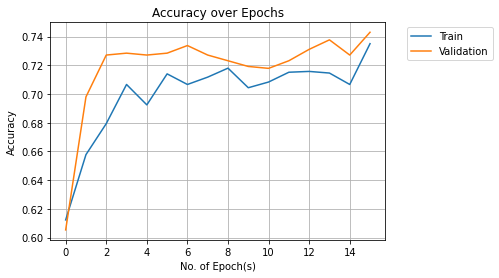
\includegraphics[width=0.5\textwidth]{accuracy-1.png}
	\caption{One Hot Encoding Preprocessor - CNN Recall}
	\label{fig:ohep-acc}
\end{figure}

\begin{figure}[h!]
	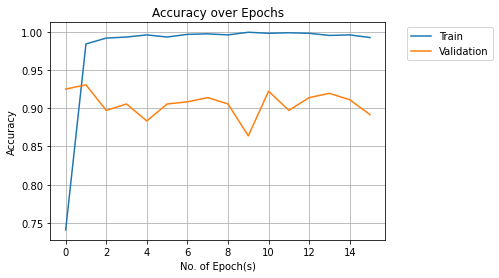
\includegraphics[width=0.5\textwidth]{accuracy.png}
	\caption{One Hot Encoding Preprocessor - CNN Recall}
	\label{fig:ohep-rec}
\end{figure}


\begin{figure}[h!]
	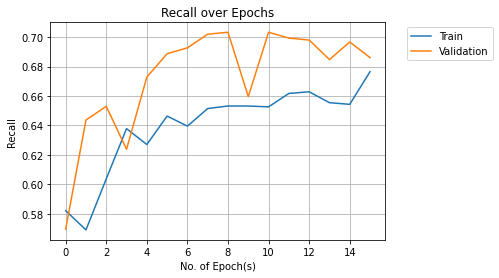
\includegraphics[width=0.5\textwidth]{recall-1.png}
	\caption{FastText Preprocessor - CNN Recall}
	\label{fig:ft-rec}
\end{figure}

\begin{figure}[h!]
	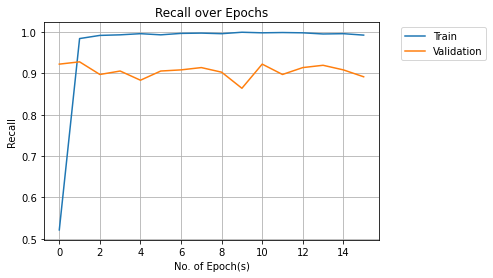
\includegraphics[width=0.5\textwidth]{recall.png}
	\caption{FastText Preprocessor - CNN Recall}
	\label{fig:ft-acc}
\end{figure}


\section{Second Implementation}

\subsection{Discussion}

\subsection{Results}

For the second implementation, we observed that in \ref{fig:ft-acc} and
\ref{fig:ft-rec}, the validation accuracy and
recall was greater than that of training accuracy. We believe this can be
attributed to the regularization we used in the model to avoid overfitting,
which includes the four dropout layers that we added. This means that the model
at validation is more general and robust, which would in turn lead to a greater
validation accuracy and recall than training.

At the first epoch, the accuracy for the validation and training data are both
approximately 0.62, while recall is 0.57 and 0.58 respectively. The accuracy
for validation then rose and hovered around 0.73, while trraining oscilated
around 0.71. In regards to recall, the validation data experienced sudden drops
at the third and ninth epochs, but otherwise rose to about 0.7, while the
training data hovered around 0.65. Let us observe the models capacity to classify
our own written descriptions in Figure 6.



\chapter{Conclusion}

Through our examinations, we have tested the efficacy of a Convolutional Neural
Network`s ability to classify descriptions of symptoms of an ailment as their
most probable diagnoses. In so doing, we created two implementations of a CNN,
one of which utilized generated training instances and One Hot Encoding while
the other used sentences from the corpus and word embeddings. Through testing
the two models ability to classify our written accounts of symptoms, we found
that the first implementation was more effective at accurately labelling
descriptions than the second. Going forward, there are several ways in which the
model can become more robust. The addition of more ailments and associated web
pages would provide more variety in the possible classifications the model can
discern.

%\bibliography{report}

\end{document}
